\chapter{DVD and Bluray Creation}%
\label{cha:dvd_bluray_creation}

This section describes how to create a blu-ray DVD, or \textcolor{red}{BD} referring to a \textcolor{red}{B}lu-ray \textcolor{red}{D}VD, and a regular DVD, or \textcolor{red}{SD} referring to a \textcolor{red}{S}tandard \textcolor{red}{D}VD.  The DVDs (plural usage of DVD means either BD or SD) created are unencrypted, unlike commercially available movie DVDs.  This Cinelerra version conceivably can create different variations of DVD/Blu-ray media but for the casual user the most standard usages are readily usable and will be described here. 

Some preliminary information follows.  For NTSC, SD media is almost always $720\times480$ interlaced (the format in the United States, US).  For PAL, SD media is almost always $720\times576$ interlaced (Europe, EU, and most of the world).  An SD can conceivably be created with a lower resolution – for example $352\times240$ MPEG-1 -- but it is not useful.  Aspect ratio for either NTSC or PAL can be $4:3$ or $16:9$.  

Frames per seconds is usually $29.97$ for NTSC and $25$ fps for PAL.  The standard SD dvd generally uses the MPEG-2 program stream with a filename extension of \texttt{m2v}.  BD blu-ray media is not normally interlaced, but you can leave it interlaced.  Blu-ray uses the MPEG transport stream which contains 1 or more program streams with a default filename extension of \texttt{m2ts}.

Requirements for creating DVDs is the hardware device to write the media on and, obviously, the blank media for either BD or SD.  When generating SD media, you will have to install \textit{dvdauthor} and for BD media, install \textit{udftools} if they are not on your system.  Also, keep in mind that to mount filesystems for creating files and to burn DVDs, you will have to be root since you have to have privileges, unless special permissions have been provided for a non-root user.  It is also highly recommended to
run the Cinelerra startup from a terminal window, instead of the icon, in order to see informative messages of how to actually write the output (at prompt: keyin \texttt{<install\_directory\_path/bin/cin}).

A warning here -- writing blu-ray BDs and  regular SDs can take a large amount of clock time.  Keep in mind that a blu-ray can contain 25 hours of viewing, so would take multiple hours to just write one.

The max disk space needed is a little over $100GB$ for $50GB$ Double Layer (DL) media or $50GB$ for a single layer BD blu-ray.  A standard SD of $4.7GB$ needs about $10GB$ disk space. You probably can get by with much less if the render for blu-ray is less than 25 hours of media.  You will need twice as much disk space as the media holds to ensure you have sufficient space for working and copying.

The most important thing you need to know about in order to get started is \textit{Format} and \textit{Scale}  in the \textit{Create dvd or bd} window.  Format settings shown in the \texttt{Set Format} window are set accordingly to an algorithm.  Basically, it will take whatever you say in the asset format.  It matches that against the known Presets available so that is what will be shown.  If the asset format doesn't match any of the Presets default formats, then that will be shown as the \texttt{User Defined} format.  In addition when you load media, the format is initially set to \texttt{same as source} so matches the source input and if that matches a known preset, then that is what is shown.  The PAL versus NTSC only comes into play when there is no known correct matching format when you attempt to create a DVD Render batch job.  It is applied when you click OK. For example, if you load up a YouTube video, it will not match any known format and will choose PAL or NTSC based on time zone.

Figure~\ref{fig:preset01} shows pulldown \texttt{Presets} in \textit{Set Format} window:

\begin{figure}[htpb]
    \centering
    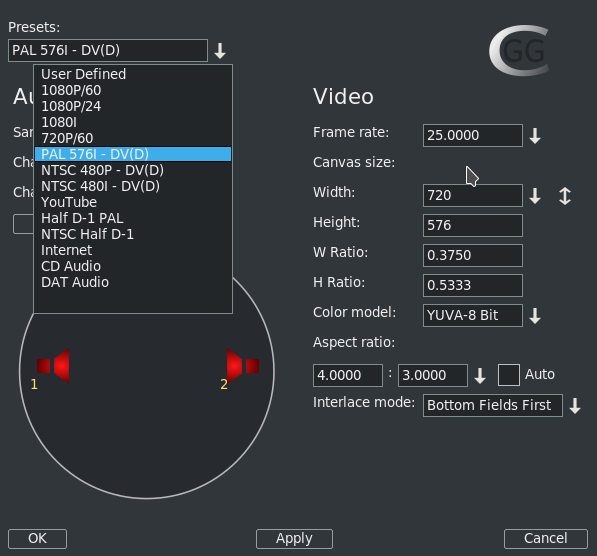
\includegraphics[width=0.7\linewidth]{images/preset01.png}
    \caption{When choose PAL, values get changed in window to reflect PAL}
    \label{fig:preset01}
\end{figure}

A quick set of basic steps to create DVDs is immediately below and usually just using the defaults will get you something.  However there is a serious issue with interaction between the Operating System and bdwrite when creating a BD/blu-ray that requires automount to be turned off.  Refer to the details and more specific explanations below the following steps for how to do this.

\begin{enumerate}
    \item If not logged in as root, you will get an error message in order to avoid doing a lot of work and then failing out because root is required for automount and to write on DVD hardware.
    \item Load your input source media via: \texttt{File $\rightarrow$ Load files}.
    \item Choose PAL or NTSC for SD/dvd or 1080P/24 for blu-ray in \texttt{Settings $\rightarrow$ Format}.
    \item For blu-ray, choose BD Render or for PAL/NTSC, choose DVD \texttt{Render} in  \textit{File} menu.
    \item Designate a \textit{work path} with sufficient disk space and then \texttt{Chk-OK}.
    \item When the Batch Render window comes up, click on \texttt{Start} and the batch jobs will run.
    \item Read the final messages echoed to the screen to see the command for burning… OR:
    \item Use the provided directory name to:\\ 
    \texttt{cd /<target directory>bd\_(or dvd\_)<date-time>}
    \item Load your media, format if needed, note device name to substitute for \texttt{<bd>} or \texttt{<dvd>}
    \begin{itemize}
        \item If rewritable blu-ray, use \\
        \texttt{dd if=./bd.udfs of=/dev/<bd> bs=2048000}
        \item If write-once blu-ray, use \\
        \texttt{growisofs -dvd-compat -Z /dev/<bd>=./bd.udfs}
        \item If any DVD media,    use \\
        \texttt{growisofs -dvd-compat -Z /dev/<dvd> -dvd-video ./iso}
    \end{itemize}
\end{enumerate}

Any problems encountered will require that you read more information in this section to include specific details, helpful hints, and problem resolution.

\paragraph{Details and specific explanations} to create blu-ray or regular DVD are provided here.  It is very advantageous to startup Cinelerra from the command line prompt instead of the icon.  Also, please be root or your hard work will be lost when the automount is issued and fails for bluray udfs mounting.

The general design of the DVD/blu-ray generation operations is to first render media using batch rendering and then terminate Cinelerra to start a script which creates the target device filesystem data.  These scripts are the \texttt{dvd.sh} and \texttt{bd.sh} scripts written into the target directory.  For DVD, the general plan is to write a directory \texttt{<target>/iso} with the dvd filesystem via \textit{dvdauthor} and then generate an iso9660 filesystem and write it to a dvd via \textit{growisofs}.  

For blu-ray, the filesystem generation is slightly harder.  First, it creates an empty filesystem image \texttt{<target>/bd.udfs} using \textit{mkudffs} which makes a big hole for the filesystem data. The hole is made just a little bigger than the data written by \textit{bdwrite} so that you don't have to write an entire $25GB$ or $50GB$ disc even if no data exists. This empty filesystem is loopback mounted to make it writable, and the linux kernel manages the filesystem image. The bdwrite program applies the blu-ray structure to the UDF filesystem by creating the needed BDMV blu-ray filesystem, which the kernel stores onto the image file \texttt{bd.udfs}.  When udfs is unmounted, the kernel finalizes the disk image on bd.udfs.  The bd.udfs image can be written directly to a blu-ray disk via \textit{dd} or \textit{growisofs}. 

NOTE of IMPORTANCE: there is a serious situation with the interaction between the Operating System (OS) and bdwrite when creating blu-ray, that requires automount to be turned off.  The blu-ray automatic script unmounts the blu-ray/UDF filesystem but the system has not finalized the directories so the OS creates a new loop file device and the data is loaded and cached for use by the new loop but it is stale.  Consequences is that not all of the data is written where it should be.  The solution is for the OS not to mount this second mount so we have to make sure it doesn't.  There are 2 methods to fix this.  The first and easiest is by using the following command to disable automount:

\begin{lstlisting}[language=bash,numbers=none]
gsettings set org.gnome.desktop.media-handling automount false
\end{lstlisting}

This can be reversed when you have completed the blu-ray generation via:

\begin{lstlisting}[language=bash,numbers=none]
gsettings set org.gnome.desktop.media-handling automount true
\end{lstlisting}

A different and more complicated method you can use to turn off automount is to download and install the \textit{dconf-editor}.  Automount is a system parameter and only needs to be done once unless you do not want automounts to always be disabled.

\begin{enumerate}
    \item run: \texttt{dconf-editor}
    \item select: org $\rightarrow$ gnome $\rightarrow$ desktop $\rightarrow$ applications $\rightarrow$ media-handling
    \item uncheck: automount
    \item close dconf-editor window
\end{enumerate}

Immediately below are the detailed steps with explanations for creating SD or BD media.

\textit{Step 1}: Construct a session with the desired presentation:

\begin{itemize}
    \item Format frame rates choices are $29.97$ or $25$ for SD, based on the user's timezone, with NTSC 29.97/US or PAL 25 /EU.  For BD, the media input will be analyzed to automatically pick the default format or if unknown, the user's timezone will be used to default to $1920/29.97i$ for US or $1920/25i$ for EU.  Be sure to set the rendering parameters in the \texttt{settings $\rightarrow$ format} menu.
    \item Choose audio stereo or 5.1, again depending on your media.
    \item Target Geometry will be $720\times480$ (US) or $720\time576$ (EU) for SD.
\end{itemize}

\textit{Step 2}: From the main window, select  \texttt{file $\rightarrow$ BD Render}   or    select  \texttt{file $\rightarrow$ DVD Render} (figure~\ref{fig:bluray_dvd}).  Then:

\begin{figure}[htpb]
    \centering
    \begin{minipage}[h]{0.49\linewidth}
        \center{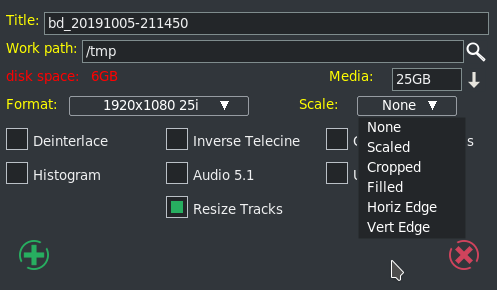
\includegraphics[width=0.99\linewidth]{images/bluray01.png}} \\ BluRay (scale pulldown)
    \end{minipage}
    \begin{minipage}[h]{0.49\linewidth}
        \center{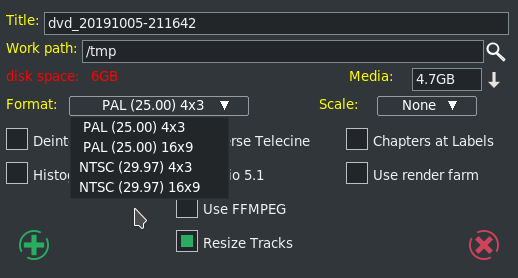
\includegraphics[width=0.99\linewidth]{images/dvd01.png}} \\ DVD (format pulldown)
    \end{minipage}
    \caption{BD Render and DVD Render}
    \label{fig:bluray_dvd}
\end{figure}

(Note: both the BD and the DVD windows above, show insufficient space, \textit{disk space:} in red)

\begin{itemize}
    \item Select desired features, check/un-check as appropriate.
    \item Click \texttt{OK} check button.  It is very important to realize that when you check OK, the EDL will be saved and that will be used for batch job rendering.  If you bring up the Batch Render and then change some parameters, they will not take effect UNLESS you remember to either check	\texttt{Save to EDL Path} or \texttt{Use Current EDL} in the Batch Render window.  You will get a reminder automatically if \texttt{warn if jobs/session mismatched} is checked.
\end{itemize}

Explanation of the choice boxes as seen in figure~\ref{fig:bluray_dvd} for both SD and BD menus is given below.  Many of them are plugins which allow you to further manipulate the settings for best results.  They are just suggestions set by the program automatically based on your input media, and can be reset to suit your needs.  These are listed in the next 4 points.

\begin{enumerate}
    \item If the media does not match the DVD target geometry, and the scale plugin is not already in use, then the \textit{scale} plugin is applied with scaling set to fit the media dimensions to the DVD format target geometry.
    \item If the video height is at least twice the DVD height and the input media is interlaced, then the \textit{deinterlace} plugin is applied with odd line sampling.
    \item \textit{Audio 5.1} will automatically be set to the wide-audio if you have 6 tracks of audio.
    \item To allow video data to be accessible and overlay properly, the track buffers are \textit{resized} to the largest track frame size in use (\texttt{Resize Tracks}). The theory behind this is to make sure to have enough memory to cover the entire presentation for transcoding.
\end{enumerate}

\noindent All of the current choice boxes are further defined immediately following.

\begin{description}
    \item[Deinterlace] remove the interlace.  Interlacing is a video scanning system in which alternating lines are transmitted so that half a picture is displayed each time the scanning beam moves down the screen.  You lose a lot and the quality is bad when you view interlacing on a progressive TV.  You might not really want to use deinterlace, because if you deinterlace non-interlaced media, it will look awful.
    \item[Scale] alter the spatial mapping of an image to increase or reduce the size; modifies the picture.  When some programs scale from $4:3$ to $16:9$ they will automatically cut off the appropriate section of the image for you.  It is necessary to keep in mind, that \textit{square pixels} is the true end goal of scaling, not the aspect ratio which could result in squished or stretched output.  More information about scaling will be provided on a subsequent page with usage of the \textit{Scale Ratio} plugin.
    \item[Histogram] remaps the color space.  The color space ranges from $0-255$ for 8-bit color values.  You can use this tool to remap the color space to use the entire space or for stretching the contrast.  Also, it lets you perform global color-correction on the image.  You can use this to correct for color screens that are \textit{too blue}, or for color Televisions that produce \textit{brownish} output, or whatever.  In addition to color-correction, you can use the RGB modification tool to add color to images that didn't have color to begin with.  For instance, you can \textit{pseudo-color} greyscale media.
    \item[Inverse Telecine] the reverse of $3:2$ pulldown where frames, which were duplicated to create 60-fields/second video from 24-frames/second film, are removed.  MPEG-2 video encoders usually apply an inverse Telecine process to convert 60-fields/second video into 24-frames/second encoded video. The encoder adds information enabling the decoder to recreate the 60-fields/second display rate. \textit{Telecine}, i.e. $3:2$ pulldown, is used to transfer film to video. That's where the $3:2$ ratio comes in. To ensure that there will consistently be 60 frames per second, the first frame is displayed on the TV screen 3 times and the second frame is displayed 2 times. The following frame is repeated 3 times, the next one 2 times, etc. throughout the film.  For inverse telecine, you show 2 of the film frames for 3 of output frames.  Only check \textit{Inverse Telecine} if you have film or something that is $24fps$ and want to project to $30fps$ (most likely this will never be necessary).
    \item[Audio 5.1] 6 channel surround sound.  For most home systems, uses five full bandwidth channels and one low-frequency effects channel.  Could automatically get set as explained previously.
    \item[Aspect Ratio] aspect ratio may be automatically set to $4:3$ or $16:9$.  Aspect ratio would better be defined as the size of the display, monitor, or TV which will be used to view the output.  If you measure your old TV, which supposedly is $4:3$ and your latest digital TV, which is supposedly $16:9$, you will see that those ratios aren't always correct anyway.  Then measure your laptop monitor, your desktop monitor, and your neighbor's, and lo and behold, the ratios don't fit either of the purported \textit{standard} aspect ratio.  Maintaining square pixels via scaling is more important in the long run.
    \item[Use FFMPEG] this is user's choice; it is recommended and faster but more difficult to modify due to numerous options. For blu-ray, ffmpeg must be used and is not an available option.
    \item[Resize Tracks] change track width and height as explained previously.  The size is adjusted to the largest frame size needed.
    \item[Chapters at Labels] without this checked, chapters markers are automatically inserted every 5 minutes.  The chapter labels can then be \textit{skipped to} when playing the DVD.  If instead, you want to put labels in at opportune times, you will have to run dvdauthor outside of Cinelerra and mark the chapter labels yourself by hand.  In that case, you should checkbox \texttt{Chapters at Labels} so that the automatic 10-minute labels are not created.  This checkbox is not currently available for blu-ray.
\end{description}

\begin{figure}[htpb]
    \centering
    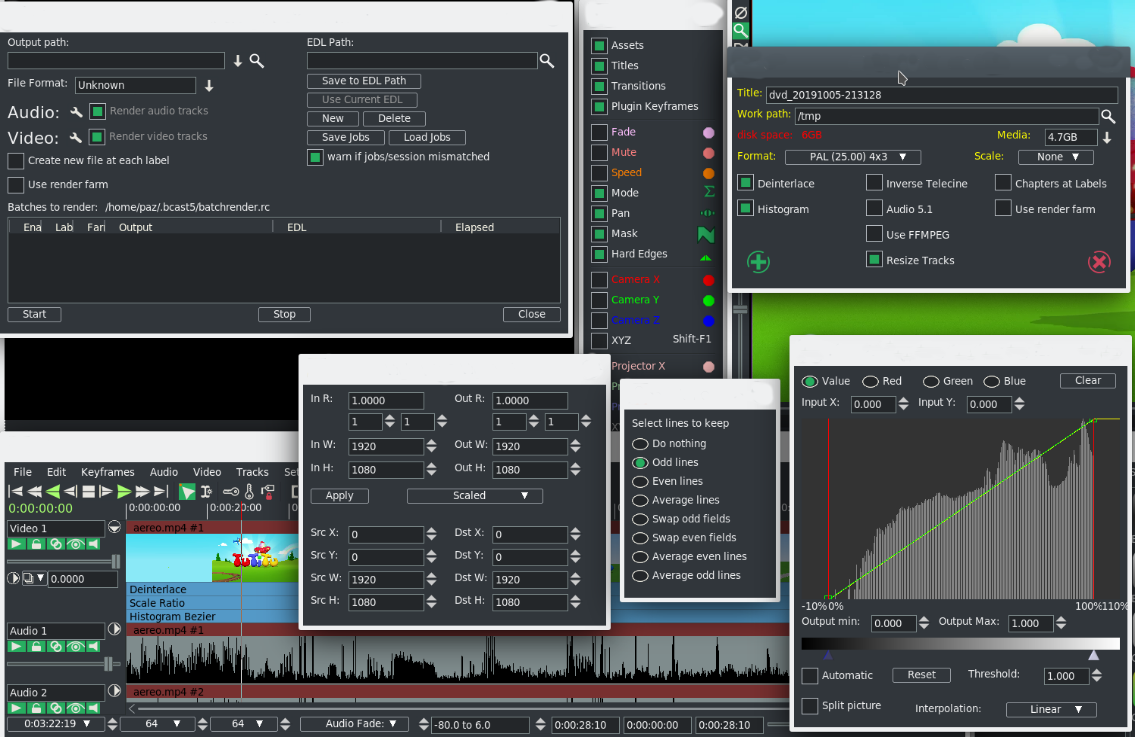
\includegraphics[width=0.9\linewidth]{images/dvd02.png}
    \caption{check Deinterlace; Histogram and Resize Tracks}
    \label{fig:dvd02}
\end{figure}

Figure~\ref{fig:dvd02} shows on the upper right side the \textit{Create DVD} window with Deinterlace, Histogram and Resize Tracks checked.  Also Scale is set to Scaled.  Once the green checkmark is clicked, the \textit{Batch Render} window comes up and in the main window you will see the 3 plugins below the video track on the main window.  By clicking on the magnifying glass that appears on the rightmost side, the controls for each will popup and you can make any necessary adjustments.  Note the numerous choices for Deinterlace; the Value, Red, Green, and Blue for color adjustments in the Histogram window; and Scale Ratio popup menu for numerical settings control.

The \texttt{Scale} parameter gives you a lot of flexibility.  A default based on your input media is provided for you but possible choices are None, Scaled, Cropped, Filled, Horiz Edge, and Vert Edge.  You will have the opportunity to manipulate the desired results in the \textit{Scale Ratio} window.  Values for W (width), H (height), and X/Y coordinates are the number of pixels.  For example, if video is $720\times432$, that is obviously 720 pixels by 432 pixels and this would be the values for Dst W and for Dst H.  So if you have some media that is off center you can crop by changing the SRC Y value AND then change DST X/Y to non-zero. It will become the output origin.  To see what it does, change them from $0.0$ to $400.0$ and you will see big changes in the compositor window.

For example, if you have the Cropped choice for the Scale, you will want to manipulate the \textit{ScaleRatio} plugin (the magnifying glass on the main window video track) which brings up the Scale window.  For cropped top instead of crop both top and bottom, modify the \texttt{Src Y}.   As you change the Y scale, you will see the cropping take place in the Compositor. 

Scaling options are provided in order to preserve image aspect ratio.  To determine which scaling option to use, it is important to correctly identify your source/destination video aspect ratios.  Next is a short explanation of possible options.

\begin{description}
    \item[None] do not do any scaling.  The destination output matches the source input.  There is no resizing.
    \item[Scaled] do not use uniform scaling on X and Y.  Just make it fit and you will might end up with squishing/stretching in one direction or the other in order to do that.  This happens when the input aspect ratio is different than that displayed on the output.
    \item[Cropped] removes outer edges of a source image in order to fit the image on the output display.  This is done in order to maintain uniform geometry scale on the destination display without being affected by the particular factor of original media aspect ratio.  Since cropping omits image area, and the areas which you wish to view may not be viewed when the image is centered, you can pan the image source using the Src X/Y to modify which area is in view.  You can also think of this as \textit{scaled up}.
    \item[Filled] the entire output display will be filled with image content but in order to do so, some of the image may have had to be cut.  Any mismatch between the two will be filled with black.  Centering of the image can be modified by using the Dest X/Y variables in the Scale Ratio controls.  You can also think of this as \textit{scaled down}.
    \item[Horiz Edge] this indicates preserving of the Horizontal edge.
    \item[Vert Edge] this option preserves the Vertical edge.
\end{description}

Horizontal and Vertical are duplicates or restatement of same functionality as Cropped or Filled but are provided as options to accommodate different ways of thinking.  In any case, you can choose which outer edges of the image to crop by using the \texttt{Show Controls} of the Scale Ratio plugin.  For example, you can ensure that no \textit{action} is lost by displaying the center of the screen only or making sure that any textual information on the bottom is not lost by cutting only the top off.

\textit{Step 3}: Batch render menu appears with \texttt{m2ts} format selected for blu-ray or \texttt{dvd} format selected for regular/standard DVD when File Format selected is ffmpeg in the previous \textit{Create DVD} menu. It will work just fine without selecting ffmpeg for DVD and may be advantageous not to.  Using the audio/video wrench tools (you will have to have the video batch job highlighted to manipulate the video or audio batch job for audio).

\begin{itemize}
    \item Setup the audio bitrate ($192000$ recommended).  Data rate is $192K$ default.
    \item Setup the video bitrate ($6000000 - 12000000$ recommended).  $10Mb/sec$ is the current default.
    \item Click \texttt{OK} check button.
\end{itemize}

The default bitrate is the largest value possible.  The actual \textit{target} bitrate is calculated based on a formula from the blu-ray/DVD code.  It divides the media size (in bits)  by the video time (in seconds) to find the bitrate that will \textit{just fit} on the target media.  This could create a weird bitrate if the media is large, and the video time is small, so the default/target bitrate is limited to $10Mb/s$.Batch jobs are then built and appended to the job list.  Once these batch jobs are built, if you make any changes, you have to start over.  You will see listed the batch jobs that are created to perform the rendering/tasks -- 2 jobs for blu-ray, one for audio/video processing and one for the scripts.  There will be 3 batch jobs created for DVD when not using ffmpeg to include one each for audio and video and then one more for the scripts.  When you click on \texttt{start}, it fires off those jobs and you will see the rendering main window progress bar in the bottom corner reflecting the fact that it is currently processing.  Be aware that the Cinelerra program will be totally shutdown AFTER the batch jobs finish.  Screenshot below shows BD blu-ray creation with 2 batch jobs queued up and ready to go.

Figure~\ref{fig:dvd-batch01} for DVD and Figure~\ref{fig:dvd-batch02} for BD shows a creation render ready to be started.  Note that because it is not ffmpeg, the processing of video is done separately from audio.  If you need to modify the video tracks, which you can see is ghosted out, you need to highlight the first batch job listed.  Be sure to highlight the first batch job before pressing Start so it runs all of the jobs and be sure the X for job enabled is set.

\begin{figure}[htpb]
    \centering
    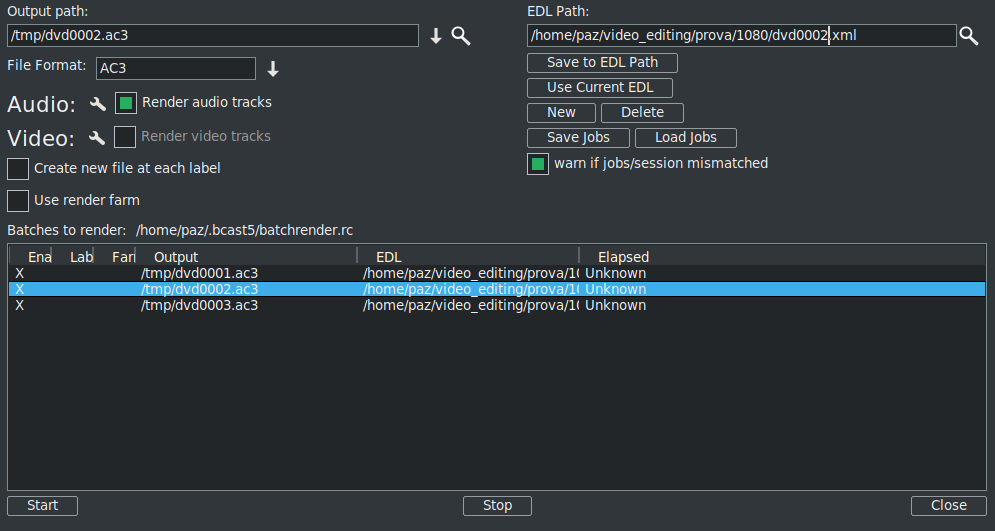
\includegraphics[width=0.8\linewidth]{images/dvd-batch01.png}
    \caption{Batch render for DVD creation}
    \label{fig:dvd-batch01}
\end{figure}

% \vspace{-4ex}
\begin{figure}[htpb]
    \centering
    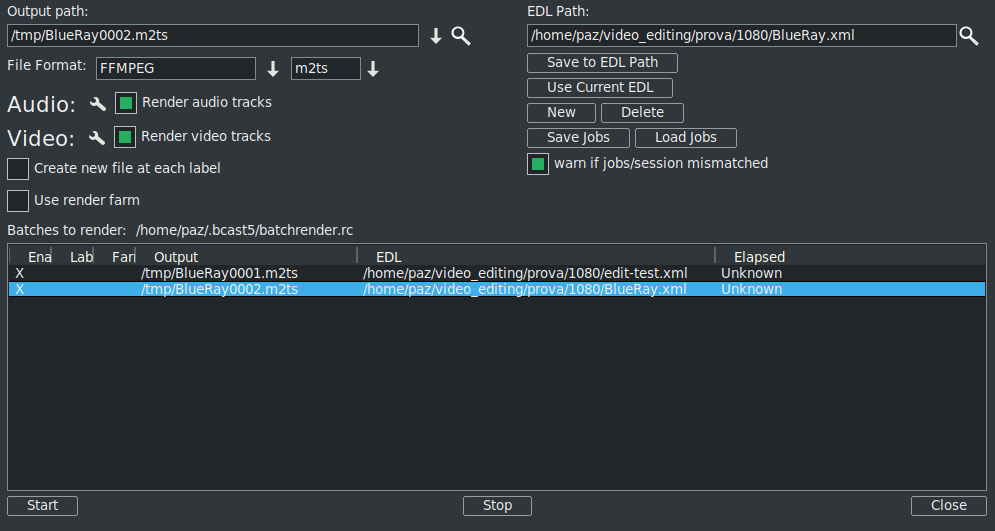
\includegraphics[width=0.8\linewidth]{images/dvd-batch02.png}
    \caption{Batch render for BD creation}
    \label{fig:dvd-batch02}
\end{figure}

When you click on \texttt{start}, it fires off those jobs and you will see the rendering main window progress bar in the bottom corner reflecting the fact that it is currently processing.  Be aware that the Cinelerra program will be \textbf{totally shutdown after the batch jobs finish} and you will be at the command line prompt.

This will produce a new directory in your target path which contains a filesystem image file.
For example: \\
\texttt{/TargetDirectory/bd\_20150820-093747} \\
Directory and file names should not be changed at this time because the scripts and programs rely on the given names in order to proceed.  You can change them later for your own purposes.

If bluray to test the filesystem you just created, use the command line interface; loopback mount the filesystem image which was generated in the target directory.  For example if blu-ray:

\begin{lstlisting}[language=bash,numbers=none]
cd /TargetDirectory/bd_20150820-093747/
mount -o loop,ro ./bd.udfs ./udfs
#check the media using a compatible media rendering tool like ffplay
umount ./udfs...
\end{lstlisting}

To burn blu-ray media you will need to run from the command line interface.  In the examples below, \texttt{/dev/bd} represents your blu-ray writer device (for example: \texttt{/dev/sr1}) and \texttt{/dev/dvd} represents your dvd writer device (for example: \texttt{/dev/sr0}).

\subsubsection*{Blu-ray Media}
\label{ssub:bluray_media}

For rewritable blu-ray (recommended) (BD-RE):

Note: unwritten (virgin) media must be formatted first using:

\begin{lstlisting}[language=bash,numbers=none]
dvd+rw-format /dev/bd   #only done once and does not take very long
\end{lstlisting}

To write or rewrite rewritable blu-ray media:

\begin{lstlisting}[language=bash,numbers=none]
cd /TargetDirectory/bd_20150820-093747/
dd if=./bd.udfs of=/dev/bd bs=2048000    #the growisofs command below also works
\end{lstlisting}

To write blu-ray write-once media: (BD-R)  (no pre-formatting needed):

\begin{lstlisting}[language=bash,numbers=none]
cd /TargetDirectory/bd_20150820-093747/
growisofs -dvd-compat -Z /dev/bd=./bd.udfs
\end{lstlisting}

\subsubsection*{DVD Media}
\label{ssub:dvd_media}

For rewritable DVD (DVD+RW):

Note: unwritten (virgin) media must be formatted first using:

\begin{lstlisting}[language=bash,numbers=none]
dvd+rw-format /dev/dvd   #only done once and does not take very long
\end{lstlisting}

To write a DVD, load blank media and run the following from the command line (requires dvdauthor):

\begin{lstlisting}[language=bash,numbers=none]
cd /TargetDirector/dvd_20160404-175416
growisofs -dvd-compat -Z /dev/dvd -dvd-video ./iso
\end{lstlisting}

Figure~\ref{fig:dvd-batch03} shows the availability of 4:2 :2 for a Batch Render seen by clicking on wrench icon.

\begin{figure}[htpb]
    \centering
    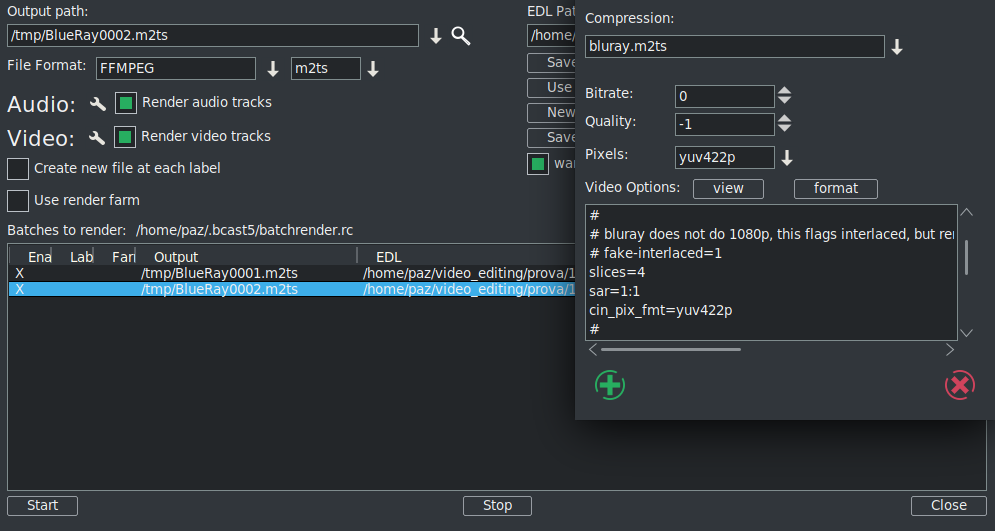
\includegraphics[width=0.7\linewidth]{images/dvd-batch03.png}
    \caption{Video options for bluray yuv422p}
    \label{fig:dvd-batch03}
\end{figure}

Figure~\ref{fig:dvd-batch04} shows the availability of 10-bit high quality 4:2 :2 for a Batch Render seen by clicking on wrench icon.  You need specially compiled Cinelerra in order to use the x265 10-bit as opposed to 8-bit.

\begin{figure}[htpb]
    \centering
    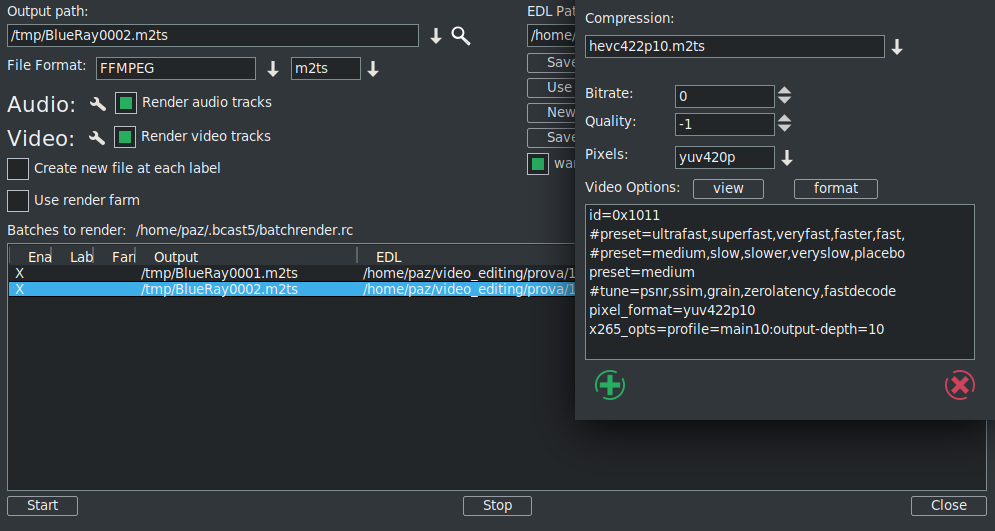
\includegraphics[width=0.7\linewidth]{images/dvd-batch04.png}
    \caption{Video options for bluray yuv422p10}
    \label{fig:dvd-batch04}
\end{figure}

\section{Output Terminal Messages from Creating DVDs}%
\label{sec:output_terminal_messages_dvd}

Below are examples of what the batch jobs generate and you will see on the terminal screen if you started the Cinelerra program in the recommended manner from a terminal window.  It is just informational but will let you know if errors.  In looking at any of the output, you can safely ignore the errors that read \texttt{Unsupported codec with id 100357 for input stream 0} -- this comes from \textit{nav-data} (navigation data).  The first 2 examples are seen from running the batch jobs; the last 2 are from the single line execution which records the media output to the DVD hardware.

\subsubsection*{SD Example: Partial Output during Cinelerra run}
\label{ssub:sd_example_partial_output}

\begin{lstlisting}[language=bash,numbers=none]
...
FFMPEG::open_decoder: some stream times estimated
Render::render_single: Session finished.
FFMPEG::open_decoder: some stream times estimated
Render::render_single: Session finished.
running /tmp/dvd_20160407-113530/dvd.sh 1 /tmp/dvd_20160407-113530
INFO: [mplex] mplex version 2.1.0 (2.2.7 $Date: 2012/11/17 01:55:16 $)
INFO: [mplex] File /tmp/dvd_20160407-113530/dvd.m2v looks like an MPEG Video stream.
. . .
INFO: [mplex] MUX STATUS: no under-runs detected.
DVDAuthor::dvdauthor, version 0.7.1. 
Build options: gnugetopt graphicsmagick iconv freetype fribidi fontconfig
Send bug reports to <dvdauthor-users@lists.sourceforge.net>

INFO: default video format is NTSC
INFO: dvdauthor creating VTS
STAT: Picking VTS 01

STAT: Processing /tmp/dvd_20160407-113530/dvd.mpg...
STAT: VOBU 32 at 15MB, 1 PGCs
INFO: Video pts = 0.133 .. 22.789
INFO: Audio[0] pts = 0.133 .. 22.789
STAT: VOBU 46 at 21MB, 1 PGCs
CHAPTERS: VTS[1/1] 0.000
INFO: Generating VTS with the following video attributes:
INFO: MPEG version: mpeg2
INFO: TV standard: ntsc
INFO: Aspect ratio: 16:9
INFO: Resolution: 720x480
INFO: Audio ch 0 format: ac3/6ch,  48khz drc, 'en'

STAT: fixed 46 VOBUs                         
INFO: dvdauthor creating table of contents
INFO: Scanning /tmp/dvd_20160407-113530/iso/VIDEO_TS/VTS_01_0.IFO
To burn dvd, load blank media and run:
growisofs -dvd-compat -Z /dev/dvd -dvd-video /tmp/dvd_20160407-113530/iso
\end{lstlisting}

\subsubsection*{BD Example: Partial Output during Cinelerra run}
\label{ssub:bd_example_partial_output}

\begin{lstlisting}[language=bash,numbers=none]
...
FFMPEG::open_decoder: some stream times estimated
Render::render_single: Session finished.
+ PATH=/usr/lib64/ccache:/usr/local/sbin:/usr/local/bin:/usr/sbin:/usr/bin:/root/bin:/mnt0/build5/cinelerra-5.1/bin
+ mkdir -p /tmp/bd_20161224-162059/udfs
++ du -sb /tmp/bd_20161224-162059/bd.m2ts
++ sed -e 's/[  ].*//'
+ sz=19811904
+ blks=13769
+ mkudffs /tmp/bd_20161224-162059/bd.udfs 13769
start=0, blocks=16, type=RESERVED 
start=16, blocks=3, type=VRS 
start=19, blocks=237, type=USPACE 
start=256, blocks=1, type=ANCHOR 
start=257, blocks=16, type=PVDS 
start=273, blocks=1, type=LVID 
start=274, blocks=13238, type=PSPACE 
start=13512, blocks=1, type=ANCHOR 
start=13513, blocks=239, type=USPACE 
start=13752, blocks=16, type=RVDS 
start=13768, blocks=1, type=ANCHOR 
+ mount -o loop /tmp/bd_20161224-162059/bd.udfs /tmp/bd_20161224-162059/udfs
+ bdwrite /tmp/bd_20161224-162059/udfs /tmp/bd_20161224-162059/bd.m2ts
+ umount /tmp/bd_20161224-162059/udfs
+ echo To burn bluray, load writable media and run:
To burn bluray, load writable media and run:
+ echo for WORM: growisofs -dvd-compat -Z /dev/bd=/tmp/bd_20161224-162059/bd.udfs
for WORM: growisofs -dvd-compat -Z /dev/bd=/tmp/bd_20161224-162059/bd.udfs
+ echo for RW: dd if=/tmp/bd_20161224-162059/bd.udfs of=/dev/bd bs=2048000
for RW: dd if=/tmp/bd_20161224-162059/bd.udfs of=/dev/bd bs=2048000
\end{lstlisting}

\subsubsection*{SD Example – Partial Output during writing disc media}
\label{ssub:sd_example_partial_output_writing}

\begin{lstlisting}[language=bash,numbers=none]
growisofs -dvd-compat -Z /dev/sr0 -dvd-video /tmp/dvd_20161224-160756/iso
WARNING: /dev/sr0 already carries isofs!
About to execute 'mkisofs -dvd-video /tmp/dvd_20161224-160756/iso | builtin_dd of=/dev/sr0 obs=32k seek=0'
I: -input-charset not specified, using utf-8 (detected in locale settings)
75.62% done, estimate finish Sat Dec 24 16:09:51 2016
Total translation table size: 0
Total rockridge attributes bytes: 0
Total directory bytes: 4096
Path table size(bytes): 42
Max brk space used 1a000
6624 extents written (12 MB)
/dev/sr0: "Current Write Speed" is 4.1x1352KBps.
builtin_dd: 6624*2KB out @ average 0.7x1352KBps
/dev/sr0: flushing cache
#
\end{lstlisting}

\subsubsection*{BD Example – Partial Output during writing disc media}
\label{ssub:bd_example_partial_output_writing}

\begin{lstlisting}[language=bash,numbers=none]
growisofs -dvd-compat -Z /dev/sr0=/tmp/bd_20161224-155658/bd.udfs
Executing 'builtin_dd if=/tmp/bd_20161224-155658/bd.udfs of=/dev/sr0 obs=32k seek=0'
/dev/sr0: "Current Write Speed" is 2.0x4390KBps.
1605632/24524800 ( 6.5%) @0.0x, remaining 1:39 RBU 100.0% UBU   0.0%
1605632/24524800 ( 6.5%) @0.0x, remaining 2:22 RBU 100.0% UBU 100.0%
1605632/24524800 ( 6.5%) @0.0x, remaining 3:05 RBU 100.0% UBU 100.0%
5865472/24524800 (23.9%) @0.3x, remaining 0:54 RBU 100.0% UBU  33.3%
11829248/24524800 (48.2%) @0.4x, remaining 0:21 RBU  75.8% UBU  37.5%
17858560/24524800 (72.8%) @0.4x, remaining 0:08 RBU  39.8% UBU  79.2%
23789568/24524800 (97.0%) @0.4x, remaining 0:00 RBU   4.5% UBU   4.2%
builtin_dd: 11984*2KB out @ average 0.2x4390KBps
/dev/sr0: flushing cache
\end{lstlisting}

\section{Debugging DVDs Creation}%
\label{sec:debugging_dvd_creation}

This section contains helpful hints, how to initially check the results, and some information on determining what might have gone wrong and how to address it.

\begin{enumerate}
    \item For first time users, taking the defaults seem to work very well when running as root.
    \item You may want to use rewritable media to see how it goes before using permanent media.
    \item Until you are familiar with the procedure, start with shorter input in order not to waste time.
    \item Test the generated output with a compatible media rendering tool before burning DVDs.
    \item Check the list of files and file sizes after the batch jobs are complete before burning DVDs.
\end{enumerate}

For blu-ray creation, \texttt{cd /workpath/bd\_date-time} directory and look for similar files:

\texttt{bd.jobs	\quad	bd.m2ts	\quad   bd.sh	\quad	bd.udfs	\quad    bd.xml}

\texttt{udfs} directory which is used as a loopback mount point

Note that the size of \textit{bd.udfs} should be larger than \texttt{bd.m2ts} because this is the final file which is actually going to be written to the disc media. It contains contents of \texttt{bd.m2ts} and all of the required disc structure.

For DVD creation, \texttt{cd /workpath/dvd\_date-time} directory and look for similar files:

\texttt{dvd.ac3 \quad	dvd.jobs \quad	dvd.m2v	\quad dvd.mpg \quad	dvd.sh	\quad	dvd.xml}
\texttt{iso} directory with VIDEO\_TS and AUDIO\_TS subdirectories of non-zero size.

Note that there will be no files in the actual AUDIO\_TS directory.

\begin{enumerate}[start=6]
    \item The \texttt{bd.sh} and \texttt{dvd.sh} files are script files that you can carefully run manually from some start point to determine where the failure occurred.  You must BE CAREFUL and know what you are doing and what directory you are in because dvd.sh contains an \texttt{rm} command and will delete files.  The script takes a command line parameter of the directory where the file was rendered to and which is usually the directory where dvd.sh or bd.sh was created.
    \item There is also a file in the same directory, called bd.jobs.  It was the information that was used in creating the batch jobs and may be helpful in determining what parameters were actually used if there are any resulting problems.  With enough background knowledge, you can make changes and rerun.
    \item For blu-ray check to make sure you do not have any spurious loopback disks mounted that may interfere with the correct generation.  Use the df command to check this and then the umount command to unmount these.  Also, check to make sure you have used the gsettings command to disable automount.
    \item For blu-ray loopback mount the \texttt{<target>/bd.udfs} image, and see if it has the BDMV filesystem written to it, and in particular a subdirectory named STREAM.  Look at the results in \texttt{./udfs} and check for  the stream file which should exist in \texttt{./udfs/BDMV/STREAM/00000.m2ts} and should have the same size as \texttt{./bd.m2ts}.
    \begin{lstlisting}[language=bash,numbers=none]
    mount -o loop <target>/bd.udfs <target>/udfs
    ls -lR <target>/udfs
    du -sc <target>/udfs
    umount <target>/udfs
    \end{lstlisting}
\end{enumerate}

\subsubsection*{Checklist for Troubleshooting}
\label{ssub:checklist_troubleshooting}

\begin{itemize}
    \item Are you logged in as root?  This is required in order to loopback mount files for bluray and to write media on \texttt{/dev/hardware}.  See section \hyperref[sec:bluray_workaround_mount_umount]{13.7} for a workaround for normal user mode.
    \item Did you startup Cinelerra from a terminal window so you can see informative messages?
    \item Is udftools installed for BD and dvdauthor installed for SD?
    \item Do you have loopback not enabled for bluray?  At least temporarily, disable automount via:
    \begin{lstlisting}[language=bash,numbers=none]
    gsettings set org.gnome.desktop.media-handling automount false
    \end{lstlisting}
    \item Did you have sufficient disk space for working/writing files?  In the \textit{Create} window, the \textit{disk space} will be displayed in green if sufficient, but in red if less than what fits on the disc media.
    \item Did you use \texttt{/tmp} as the work device, then rebooted the computer, which deleted files on \texttt{/tmp}?
    \item If the input media is interlaced, did you check the Deinterlace option to eliminate interlacing?
    \item Did you change the output name in the \textit{Batch Render} window after the batch jobs were already created? These filenames have already been written to disk. If you want to change either the Title or the \texttt{Work\_path}, you have to start over.
    \item Have you selected a Title in the Create window that is a directory that already exists? The program attempts to create that directory and will give you an error message if it exists.
    \item Did you replace the \texttt{/dev/bd} or \texttt{/dev/dvd} on the command line with your hardware device name?
    \item If a warning was issued in the Create BD/SD window of \textit{* non-standard format} and your bluray reader could not play the disc, did you change to a standard format instead?
    \item Did you correctly interpret the frame rate if using interlaced format to be $\frac{1}{2}$ due to interlacing?
\end{itemize}

\section{Subtitles}%
\label{sec:subtitles}

DVD (not blu-ray... yet) subtitles are added by using the main window pulldown   \texttt{File $\rightarrow$ Subtitle}   which brings up a window allowing you to type the filename of a previously generated text file containing the desired words/lines, the script.  After entering the filename, click \texttt{Load} to read in your script.  By creating a script file ahead of time, it lets you easily add dialog that was already written out and carefully edited for spelling and proper grammar.

The format of the script/text input file has specific requirements as listed below:

\begin{itemize}
    \item Lines can be any length but they will be broken up to fit according to some criteria below.
    \begin{itemize}
        \item Running text used as script lines will be broken into multiple lines.
        \item The target line length is 60 characters.
        \item Punctuation may be flagged to create an early break.
        \item Single carriage return ends an individual script line.
        \item Double carriage return indicates the end of a entry and helps to keep track of where you are.
    \end{itemize}
    \item The "\textit{=}" sign in column 1 indicates a comment seen in the script text to assist you in location.
    \item An “\textit{*}” at the beginning of the line is a comment and not a script line.
    \item \textit{Whitespace} at either the beginning of a script line or the end will be removed.
\end{itemize}

Figure~\ref{fig:subtitle01} shows the Subtitle window you will see.

\begin{figure}[htpb]
    \centering
    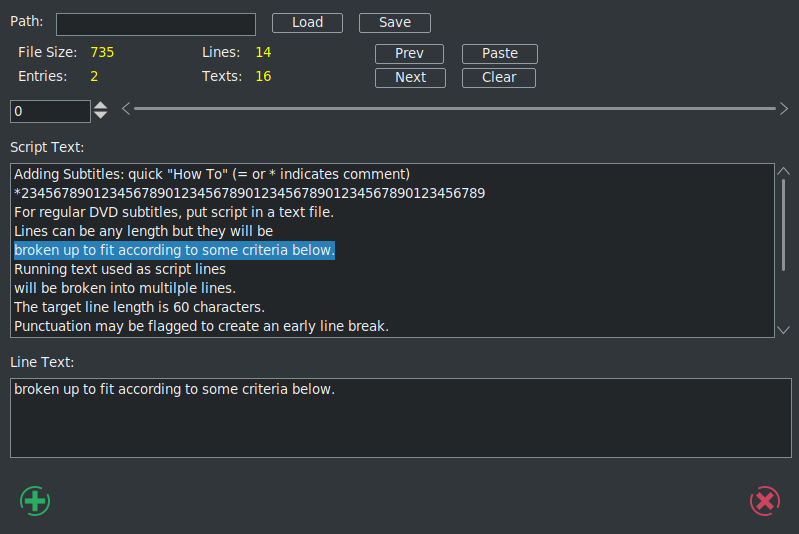
\includegraphics[width=0.8\linewidth]{images/subtitle01.png}
    \caption{Subtitle window}
    \label{fig:subtitle01}
\end{figure}

To put the subtitles onto your media, first add a subtitle track via the pulldown  \texttt{Track $\rightarrow$ Add Subttl}. In the Subtitle window, note that there are 2 major textboxes.  There is the \textit{Script Text} textbox showing the current entry of text from your input file and there is the \textit{Line Text} textbox showing the currently active text.  In your subtitle track, select a timeline region (in/out or drag select with hairline cursor/highlight) to indicate the region where you want the active Line Text to be pasted.  Then click the \texttt{Paste} button in the Subtitle window to paste the line onto the subtitle track.  Silence will be added to the subtitle track in the places in the media where there are gaps.

Editing in the Line Text box can be used to change the active script line. By double clicking the timeline over the subtitle track, you can reselect the active script line.  The subtitle text will be reloaded into the Line Text box and can be edited and re-pasted as the new active subtitle text.  You can also highlight multiple lines in the Script Text box and paste them (using the usual window paste methodology) into the Line Text box.  After pasting to the timeline, the Line Text box will be updated with the next script line.  In addition, if you triple click a line in the \textit{Script Text} box, it will automatically become the current line in the \textit{Line Text} box.

When you are finished, before clicking \texttt{Save}, you must supply a legitimate filename in the \textit{Path} box; your current directory will be used if only a filename but no directory path is supplied.  The filename used will automatically have a “-” after it followed by the \textit{track label} and then \textit{udvd} extension added; any extension in the filename will be removed..  If you click \texttt{OK} before saving, the subtitle script position is saved with the session.  This is convenient for continuing where you left off.

\noindent To reposition the script, use the slider or tumbler buttons:

\textit{Slider} bar to move through the text entries quickly.

\textit{Prev} or \textit{Next} buttons to go to the previous or next script line.

\noindent Figure~\ref{fig:subtitle02} shows what the pasted subtitle script looks like in a portion of the main window.

\begin{figure}[htpb]
    \centering
    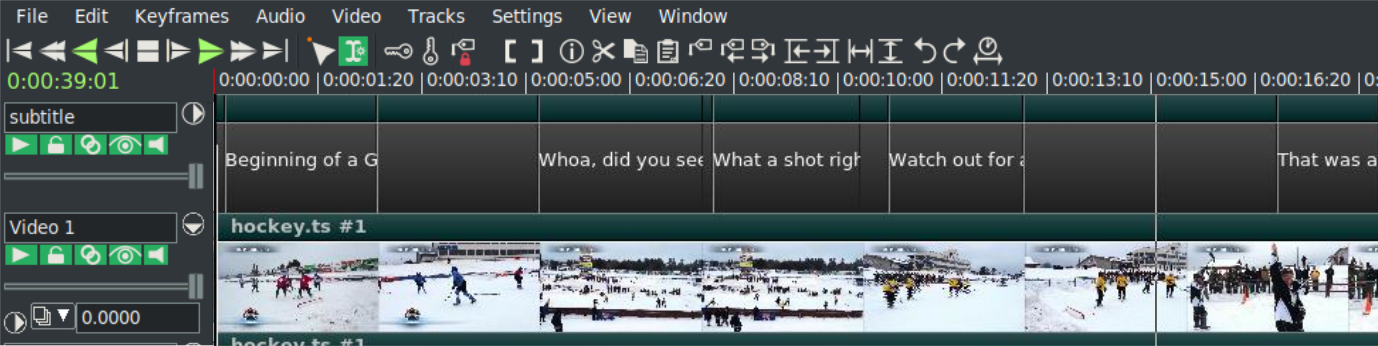
\includegraphics[width=0.9\linewidth]{images/subtitle02.png}
    \caption{Subtitles on timeline}
    \label{fig:subtitle02}
\end{figure}

\section{Dvd Interlaced Chroma}%
\label{sec:dvd_interlaced_chroma}

Cinelerra uses $4:4:4$ colorspace to edit, so it is necessary to convert interlaced $4:2:0$ video to $4:4:4$.
But you can run into problems, referred to as the \textit{chroma bug}, which you see in DVD media displayed on higher resolution monitors -- streaks or spiky horizontal lines are visible in the chroma channel, especially on diagonal edges. The Chroma Bug is specific to MPEG and 4:2:0 encoding.

Now you can use the \textit{YUV420P DVD Interlace Mode} when rendering DV directly to mpeg2 through a yuv4mpeg stream and when using video effects on HDV video.

With this option enabled, improved chroma results will be obtained from your DV or HDV source.
Editing DV or HDV and rendering it back to the same format does not require any special handling.
In order to perform colorspace conversions correctly in Cinelerra and avoid Chroma errors for interlaced $4:2:0$ video, check the box as follows:

\texttt{Settings $\rightarrow$ Performance $\rightarrow$ YUV420P DVD Interlace Mode}

This option maintains the interlacing in Chroma sample addressing, which ordinarily would be deleted
because the upsampling of interlaced chroma fields is normally done using a progressive algorithm.
With this mode enabled, the MPEG decoder uses a different algorithm for interlaced frames so that the
$4:2:0$ format chroma interlacing is preserved.

\section{MPEG utility programs}%
\label{sec:mpeg_utility_programs}

There are 2 utility programs that come in handy when dealing with DVD media for creating or reading previously written DVDs.

\paragraph{zmpeg3cc2txt} convert closed captioning data to subtitle data.

This program can be used to scan captured broadcast data streams and convert the closed captioning text data into subtitle track data.  The result can be used to add subtitles to DVDs created from the captured media using the text collected from the closed captioning.

usage:

\begin{lstlisting}[language=bash,numbers=none]
./zmpeg3cc2txt  [-c cc_service ]  [-s start:length, ...]  [ -t track ]  [-v verbose ] [-w wdw mask ]  [-x file.xml ]  [-o file.udvd ]  file.ts
\end{lstlisting}

\begin{tabular}{lcl}
    cc\_service&=&closed caption service id\\
    
    start:length&=&start:length frames (comma separated list)\\
    
    track&=&video track number\\
    
    verbose&=&verbose level\\
    
    wdw mask&=&bit mask for windows (-1 = all)\\
    
    file.xml&=&filename for edl xml format subtitle data\\
    
    file.udvd&=&filename for udvd format subtitle data\\
    
    file.ts&=&filename for transport stream\\    
\end{tabular}

To use this program, the input file must be a transport stream (broadcast video) which contains closed captioning services.  The service id defaults to one, and the default video track is zero.  Either \texttt{-o} or \texttt{-x} must be specified to indicate the output file format desired.  If the output file name is a '-' then stdout is selected as the output file. 
For example:

\begin{lstlisting}[language=bash,numbers=none]
zmpeg3cc2txt -o - /dvb_data/channel5.ts
\end{lstlisting}

\paragraph{zmpeg3ifochk} check DVD \texttt{ifo} file for usable features.

For some time, DVD manufacturers have been employing  a variety of measures to make reading a DVD difficult on a computer.  One technique which is widely deployed is to add a bunch of extra program data, so that correct playback is only likely if you can read the DVD virtual machine data and decode a maze of program data to find the undamaged stream definitions.  Only a few streams are created which are machine usable, and dozens are created as decoy streams.  The decoy streams fail or introduce errors.  This program scans the IFO (info file) playlists and verifies the contents of the stream that does not contain obvious damage.  The result is a list of program ids which can be entered into the playback preferences to select a program which qualifies.

\section{HDV on a Blu-ray Disc Without Re-encoding}%
\label{sec:hdv_bd_without_reencoding}

An MTS file is a video file saved in the high-definition (HD) MPEG Transport Stream video format, commonly called \textit{AVCHD}.  It contains HD video compatible with Blu-ray disc format and is based on the MPEG-2 transport stream.   MTS files are often used by Sony, Panasonic, Canon and other HD camcorders.  Legal input for Video --- MPEG1VIDEO, MPEG2VIDEO, H264; Audio --- MP1, MP2, AC3, AC3PLUS, DTS, TRUHD. 

For creating a blu-ray disc, if you have HDV MPEG-2 media that is in blu-ray format, you can save the original quality of your work, rather than rendering it to another format.  Follow the steps below directly instead of going through Cinelerra.  It has been tested on 10 different MTS files.

\begin{lstlisting}[language=bash,numbers=none]
du -sb /yourHDVfile.MTS		# Determine the size of your file in bytes.
blocks=((size-in-bytes/2048 + 4096))	# Convert bytes into blocks + a little more.	
mkudffs /tmp/newfilename.udfs blocks	# Create a file with that \# of blocks + some extra.
mount -o loop /tmp/newfilename.udfs /mntX          # Use a mount point like mntX that is not in use.
/<cinelerra_installed_path>/bin/bdwrite /mntX /tmp/yourHDVfile.MTS   # Substitute Cinelerra path.
umount /mntX				# You must unmount the udfs filesystem
growisofs -Z /dev/bd=/tmp/newfilename.udfs   # Replace /dev/bd with your bluray hardware device.
OR  dd if=/tmp/newfilename.udfs of=/dev/bd bs=2048000   # if using rewritable blu-ray; replace bd.
\end{lstlisting}

\section{Blu-ray Workaround for Mount/Umount}%
\label{sec:bluray_workaround_mount_umount}

Creating BD images to be written to media requires usage of \textit{mount} and \textit{umount} which typically can only be done by the root user due to security.  If you want to avoid running Cinelerra as root, you can implement a workaround by adding a line in \texttt{/etc/fstab} (must be root to edit the file initially) and by creating a directory in your home area, called \texttt{bluray}.  You only have to do this once unless you upgrade the Operating System and it wipes out the line in \texttt{/etc/fsta}b.  Now the Cinelerra program will automatically do the mount and umount for you each time you execute BD Render and you can run as an ordinary user.

The line to add to \texttt{/etc/fstab} will look something like the following, assuming your username is \textit{name} and your groupid may be \textit{users} or \textit{name}.  If you do an \texttt{ls -l} in your home directory, the $3^{rd}$ and $4^{th}$ fields shown will be your uid or name and gid or groupid which you must substitute in the line below.

\begin{lstlisting}[language=bash,numbers=none]
/home/name/image  /home/name/bluray  udf noauto,loop,rw,user,uid=name,gid=groupid 0 0
\end{lstlisting}

Also, be sure to do a \texttt{mkdir bluray} in your \texttt{/home/name} directory as this is a requirement (owned by you; uid=gid=name).  When the actual image to be written to disc media is created, it will first d any current \texttt{/home/name/image} file.  Warning – make sure you do not already have a file called \textit{image} that you want to save as it will be automatically deleted every time you initiate a BD Render.  So you will want to burn a bluray disc after Cinelerra creates the \textit{image} since it will written over on the next rendition.  The actual writing to your bluray burner (something like \texttt{/dev/sr0}) is done outside of Cinelerra at a terminal prompt and requires root privilege usually.  You can either use \textit{sudo} for 1 line or create user wheel group to get around this.

\section{Blu-ray from Multiple Cinelerra Output}%
\label{sec:bluray_multiple_cinelerra_output}

Writing prepared multiple Cinelerra output files, \texttt{bd.m2ts}, to a single bluray disc is relatively easy to do but is not done automatically.  You can render all of the desired files via the Create BD menu, save each individual \texttt{bd.m2ts} file with a unique name, construct a Menu Title that reflects the contents of each of these files, then manually use a few commands to create a udfs file to be written to BD.

Usage of the final preparation taken from the bdwrite program comments:

\begin{lstlisting}[language=bash,numbers=none]
./bdwrite <tgt_dir_path> <playlist-0> <sep> <playlistp1> <sep> ... <sep> <playlist-n>

<sep> == -<pgm_pid> | --<pgm_pid> | ---<pgm_pid>
<pgm_pid> may be empty string, or a numeric pgm_pid for current title clip
<pgm_pid> defaults to first pgm probed
<playlist-x> == <clip-0.m2ts> <clip-1.m2ts> ... <clip-n.m2ts>
\end{lstlisting}

One title is built for each playlist; playlist-0 is used as first-play item.  The separators (\texttt{<sep>} represented by the dash character) have unique roles.  The double “$--$” means stop after playing, and the triple “$---$” means pause.

For example:

\begin{lstlisting}[language=bash,numbers=none]
./bdwrite /tmp/dir /path/menu_titles.m2ts --- /path/clip0.m2ts -- /path/clip1.m2ts -- /path/clip2.m2ts
\end{lstlisting}

The basic idea is to use playlist-0 as a menu or directions to use the bluray player remote control to select the desired Title and start the play, avoiding the need for a menu system.  Planning in advance to get the desired results is necessary.  The following steps provide an outline to get started.

\begin{enumerate}
    \item Create all of the \texttt{bd.m2ts} files that you want to put on the Bluray.
    \item Using Cinelerra, design your Title page using a few seconds of video and the \textit{Title} plugin.
    \item Use BD Create to render your short Title video.
    \item Next is the most complicated part which is to run \texttt{mkudffs} with a sufficient amount of disk space to hold all of the \texttt{bd.m2ts} files \textit{plus a little more!}  To calculate this, you can record the sizes from having run BD Create mkudffs.  This number is displayed on the terminal screen when using the command line interface each time and add them together.  Or recalculate the size of each bd.m2ts using the formula below and adding them all together.  This is the number of blocks used to make a bluray image space for bdwrite to use.  For many files, this could require a huge amount of space, so check first.
    \begin{lstlisting}[language=bash,numbers=none]
    Total size = File0 size in bytes / 2048 + 4094  "+"   File1 size in bytes / 2048 + 4094  "+" ...
    \end{lstlisting}
    Now create the image file via:   \texttt{mkudffs image <Total size>}  where image or udfs is the image name.
    \item Loop mount the disk image (refer to Section \hyperref[sec:bluray_workaround_mount_umount]{13.7}).
    \item Then actually write your multiple bd.m2ts type files onto the \textit{image} where \texttt{<cin\_path>} is the location of the Cinelerra binary \textit{bdwrite} file and \texttt{<path>} is your directory path.  Below is a single line that wrapped around with 4 Titles.
    \begin{lstlisting}[language=bash,numbers=none]
    <cin_path>/bin/bdwrite image /<path>menu_titles.m2ts --- /<path>/bd1.m2ts -- /<path>/bd2.m2ts -- /<path>/bd3.m2ts -- /<path>bd4.m2ts
    \end{lstlisting}
    Note that the 3 dashes after the \texttt{menu\_titles.m2ts} lets the bluray player know to \textit{pause} after playing the few seconds video which contains the index to the rest of the files.  The 2 dashes after each of the bd.m2ts signify \textit{stop}.  That is when you will have to use your remote to \textit{Search Titles} in order to play the next one you want to see.  In addition, if for some reason you just want to \textit{play all}, you will have to add another line to the Title menu as a choice and list all of the 4 files in a row at the end of your bdwrite line without any dashes in between.
    \item Umount the loopback disk.
    \item Use your favorite \textit{dd} or \textit{growisofs} tool to write to a formatted bluray disc.
\end{enumerate}

Figure~\ref{fig:dvd-title} demonstrates  an example of setting up a Title menu on a 5 second video.  There is a list of 4 menu title options that can be searched via remote control using the Title search option for your player.

\begin{figure}[htpb]
    \centering
    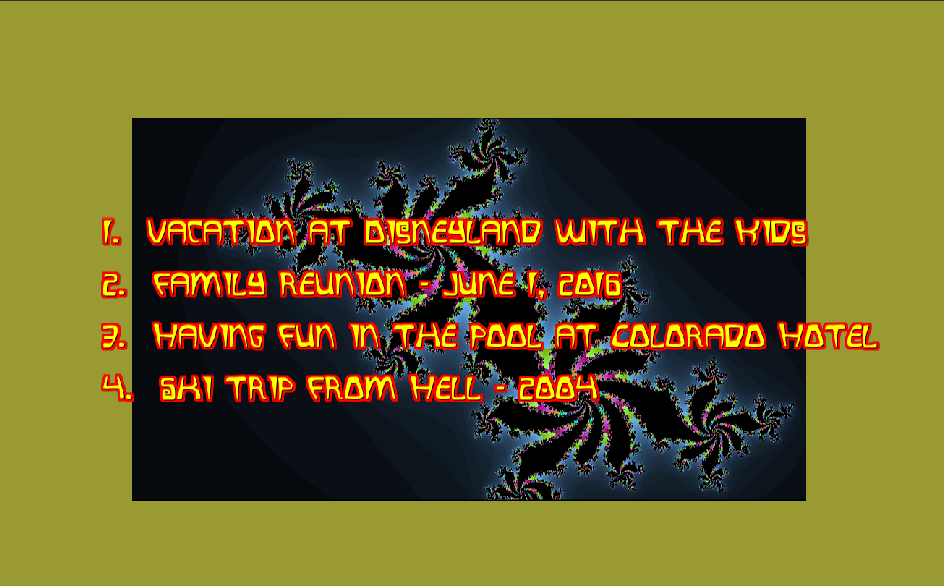
\includegraphics[width=0.8\linewidth]{images/dvd-title.png}
    \caption{Title menu for DVD/BD}
    \label{fig:dvd-title}
\end{figure}

\section{Use Case: DVD}%
\label{sec:use_case_dvd}

Example of Video Source with 4:3 Aspect Ratio, Being Transcribed to 16:9 and Creating a DVD to be Displayed on a Digital TV. Illustrated steps to take source input with 4:3 aspect ratio and convert to 16:9, with the bottom of the image being cropped in order to preserve top of video so nobody's head gets cut off are provided here.

\begin{enumerate}
    \item In order to write to a DVD writer hardware device, you must be \textit{root}!!
    \item Start Cinelerra-GG to bring up the 4 usual screens with main track canvas in the lower left corner.
    \item Load media via the pulldown \texttt{File $\rightarrow$ Load files}\dots by choosing the directory path with the desired file.
    \item Bring up the \textit{Create DVD} window using \texttt{File $\rightarrow$ DVD Render}. 
    \item Choose Format: PAL or NTSC with 16x9 aspect ratio for today's digital TV as in below screenshot. figure~\ref{fig:dvd-000}.
\end{enumerate}

\begin{figure}[htpb]
    \centering
    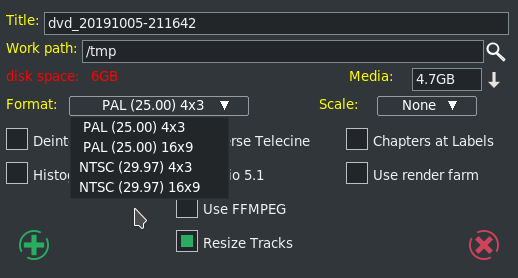
\includegraphics[width=0.7\linewidth]{images/dvd01.png}
    \caption{Choose NTSC or PAL for DVD creation}
    \label{fig:dvd-000}
\end{figure}

\begin{enumerate}[start=6]
    \item Modify the \textit{Work path:} parameter to a disk that has sufficient disk space and you will see the
    amount of disk space in green letters (\texttt{/tmp} is default, but is often deleted so may be a bad choice).
    \item Note that in the following screenshot, Scale of \textit{Cropped} has been chosen (figure~\ref{fig:dvd03}).    
\end{enumerate}

\begin{figure}[htpb]
    \centering
    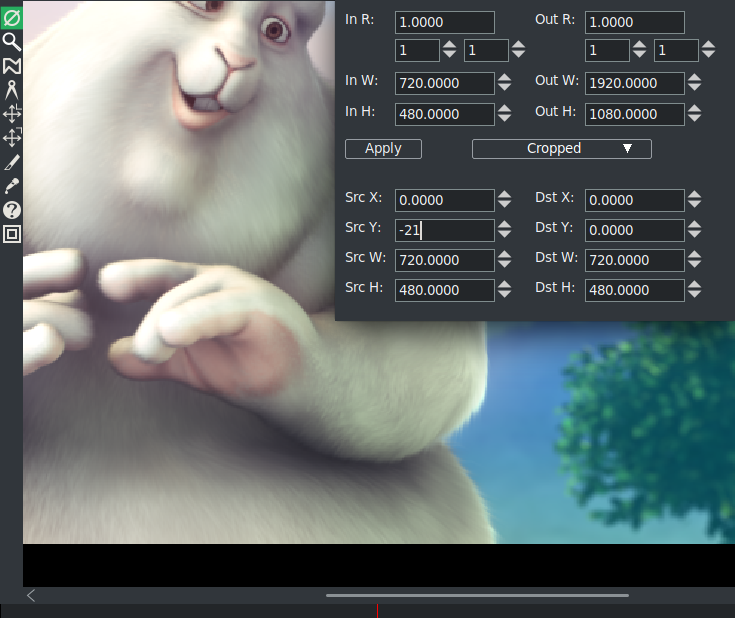
\includegraphics[width=0.9\linewidth]{images/dvd03.png}
    \caption{Set Scale Ratio to Cropped}
    \label{fig:dvd03}
\end{figure}

\begin{enumerate}[start=8]
    \item Click the green checkmark on the bottom left side of the window to close it and proceed.
    \item Now the \textit{Batch Render} window will appear along with the Scale Ratio brown-colored line below the video in the main track canvas as seen in the screenshot below. Note that in this screenshot the top right most corner of the shot displays the bottom portion of the Compositor window.
    \item Next, right mouse click the gold-colored magnifying glass, which is on the right hand side of the brown-colored line. This will bring up the Scale Ratio window that you can see below.  Note in the Compositor window, the blue legs are only showing up to the knees.
\end{enumerate}

With the \textit{Scale Ratio} plugin you can manipulate your video so that it will look the way you want it on a different output Display device.  In this case we are going to create a DVD for playing on a Digital TV screen. 

In figure~\ref{fig:scaleratio}, the left side shows the Input Ratio, Width, and Height of input. The top right half shows desired output values.  In this particular case, the input was a YouTube video which was not quite $4:3$ aspect ratio.

\begin{figure}[htpb]
    \centering
    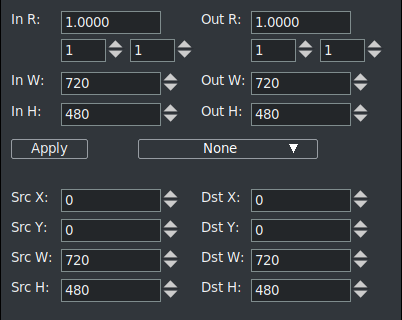
\includegraphics[width=0.7\linewidth]{images/scaleratio.png}
    \caption{Scale Ratio plugin}
    \label{fig:scaleratio1}
\end{figure}

Left and right sides of the bottom portion show the Source and the Destination X, Y, W, H values.  As you change the values on the left side, you can see how this will affect the output as you observe the results in the compositor window.  For example, as you change the values for SrcY in a \textit{cropped} Scale scenario, you see up/down movement.

Keep in mind that the monitor you are using is NOT the intended output display device --- your digital TV is, which most likely will have different looking aspect/pixels, etc.

\begin{enumerate}[start=11]
    \item In order to \textit{crop} the bottom of the video in order to preserve all of the image on the top, modify the Src Y value on the bottom of  the left hand side in the Scale Ratio plugin.  Src Y which was $21$ has now been changed to $-18$.  You will see in the Compositor window how the bottom dark colored border is now gone so that none of the top portion which contains a person's head will be chopped off. Compare figure~\ref{fig:dvd04} to figure~\ref{fig:dvd03} and note the blue legs can be now seen to the waist.
\end{enumerate}

\begin{figure}[htpb]
    \centering
    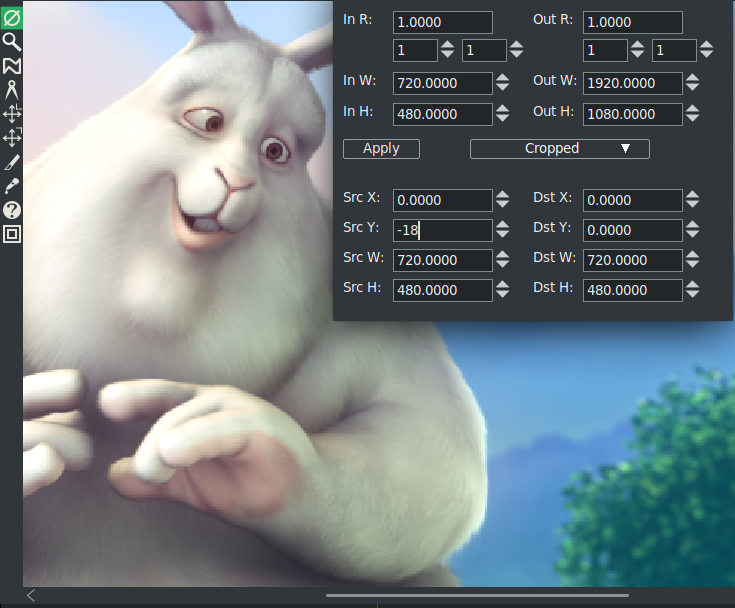
\includegraphics[width=0.9\linewidth]{images/dvd04.png}
    \caption{Better scale on compositor}
    \label{fig:dvd04}
\end{figure}

\begin{enumerate}[start=12]
    \item Click the \texttt{Apply} box in the Scale Ratio window.
    \item Click the \texttt{Save to EDL Path} in the \textit{Batch Render} window for creating a DVD.  If you do NOT do this, you will get a Warning box as seen in figure~\ref{fig:dvd-batch05}, to remind you to Save because you have changed the EDL by modifying the scaling parameters in the Scale Ratio window.
\end{enumerate}

\begin{figure}[htpb]
    \centering
    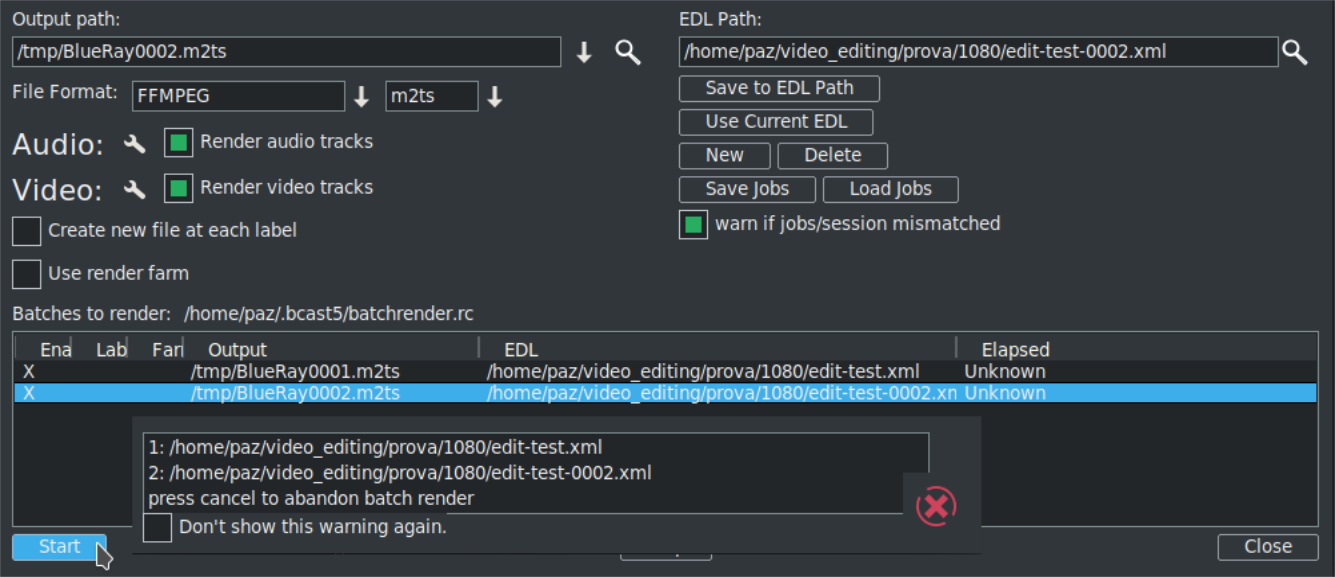
\includegraphics[width=0.8\linewidth]{images/dvd-batch05.png}
    \caption{Error in Batch Render}
    \label{fig:dvd-batch05}
\end{figure}

\begin{enumerate}[start=13]
    \item Next, make sure you have the Timeline set in the Main window at the beginning of where you want to start rendering.  Also, make sure the first line in the \textit{Batches to render} section is highlighted as you can see above by the blue highlighting.  Click on the \texttt{Start} box in the Batch Render window and you will see the video playing in the Compositor window.
    \item Cinelerra program will be stopped when done rendering; you will be at the terminal prompt where you will see it has printed out some informational messages (or errors if problems), the last 2 are:
    \begin{lstlisting}[language=bash,numbers=none]
    To burn dvd, load blank media and run:
    growisofs -dvd-compat -Z /dev/dvd -dvd-video /mnt0/dvd_20161027-131723/iso
    \end{lstlisting}
    \item Load a blank or rewritable DVD into your DVD writer device, which will be similar to \texttt{/dev/dvd} as in the \textit{growisofs} line above --- something like \texttt{/dev/sr0} on your computer.
    \item Keyin the \textit{growisofs} line, substituting your actual writer device name.  Again, you must be root.
    \item When back at the terminal prompt, and if there are no errors, keyin \texttt{eject /dev/dvd} substituting.
    \item Play it on your DVD player connected up to your Digital TV screen.
\end{enumerate}



